\scanpage{14}
\[
\begin{gathered}
\sigma_i s_j=\begin{cases}s_j&\text{si }j<i\\s_{i+1}&\text{si }j=i\\s_i&\text{si }j=i+1\\s_0+\lambda_{i,1}e_1+\ldots+\lambda_{i,i+1}e_{i+1}+\lambda_{i,i+2}e_j&\text{si }i+2\leq j\leq n+1\end{cases}\\
(0\leq i\leq n\quad0\leq j\leq n+1)\qquad(\text{donc }0\leq i\leq n-1)
\end{gathered}
\]
\[
\begin{gathered}
\sigma_i e_j=\begin{cases}e_j&\text{si }j<i\\e_{i+1}&\text{si }j=i\\e_i&\text{si }j=i+1\\\lambda_{i1}e_1+\ldots+\lambda_{i,i+1}e_{i+1}+\lambda_{i,i+2}e_j&\text{si }i+2\leq j\leq n+1\end{cases}\\
1<i\unsure{\leq|<}n\qquad(\text{donc }0\leq i\leq n-1)
\end{gathered}
\]
\[
\sigma_0e_j=\begin{cases}-e_1&\text{si }j=1\\(\lambda_{0,1}-1)e_1+\lambda_{0,2}e_j&\text{si }2\leq j\leq n+1\end{cases}
\]
\[
\sigma_0^2=\mathrm{id}\quad\Longleftrightarrow\quad\left\{\begin{aligned}(\lambda_{01}-1)(\lambda_{02}-1)&=0\\\lambda_{02}^2&=1\end{aligned}\right.
\]
\[
\begin{gathered}
\sigma_i^2=\mathrm{id}\quad\Longleftrightarrow\quad\left\{\begin{aligned}
\lambda_{i1}(1+\lambda_{i,i+2})&=\lambda_{i2}(1+\lambda_{i,i+2})=\cdots=\lambda_{i,i-1}(1+\lambda_{i,i+2})=0\\
\lambda_{i,i+1}+\lambda_{i,i+2}\lambda_{ii}&=\lambda_{i,i}+\lambda_{i,i+2}\lambda_{i,i+1}=0\\
(\lambda_{i,i+2}^{\deleted{\unsure{2}}})^2&=1
\end{aligned}\right.\\
(1\leq i\leq n-\unsure{1})
\end{gathered}
\]
\margin{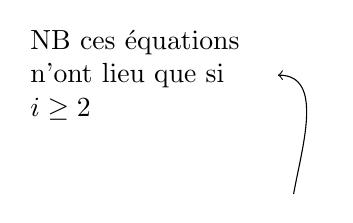
\begin{tikzpicture}
\node[text width=3.1cm,inner sep=1pt] (note) at (0,0) {\uline{NB} ces équations \unsure{n'ont} lieu que si $i\geq2$};
\draw[->] ([xshift=2mm,yshift=-9mm]note.south east) to[out=80,in=0] (note.east);
\end{tikzpicture}}
% The marginal arrow refers to the first line of the preceding brace.

$\sigma_n^2=\mathrm{id}$ tjrs vérifié, $\sigma_n$ est une \uline{réflexion}

Exprimons que $\sigma_0$ est une réflexion.

\[
\deleted{\sigma_0=\left(\begin{array}{ccccc}-1&\lambda_{01}-1&\lambda_{01}-1&\ldots&\unsure{\lambda}\\0&&&&\\\vdots&&&&\\0&&&&\end{array}\right.}
\]
\[
\deleted{\sigma_0(x_1,\ldots,x_{n+1})=\sigma_0(s_0+x_1e_1\ldots+x_{n+1}e_{n+1})}
\]
\[
\deleted{\sigma_0=}
\]
\[
\sigma_0=\left(\begin{array}{cccccc}
-1&\lambda_{0,1}-1&\lambda_{0,1}-1&\ldots&\lambda_{01}-1&1\\
0&\lambda_{0,2}&0&&0&0\\
0&0&\lambda_{02}&&0&0\\
\vdots&\vdots&\vdots&&\vdots&\vdots\\
0&0&0&&\deleted{\unsure{0}}\lambda_{02}&0\\
0&0&0&&\deleted{\unsure{\lambda}}0&1
\end{array}\right)
\]
\[
\underbrace{\hspace{7cm}}_{n+1}
\]
% The underbrace spans the first n+1 columns.
\[
\begin{aligned}
\sigma_0(x_1,\ldots,x_{n+1})&=\deleted{\unsure{(1-x_1,(\lambda_{01}-1)+}}\\
&(1-x_1+(\lambda_{0,1}-1)(x_2+\ldots+x_{n+1}),\lambda_{0,2}x_2,\ldots,\lambda_{0,2}x_{n+1})
\end{aligned}
\]
% archive sheet number: 13
